\chapter{Funcionalidades do MDArte}

Neste capítulo iremos explorar algumas funcionalidades que já existem no MDArte,
a fim de agilizar e simplificar o processo de desenvolvimento. Para tal
alteraremos os modelos de \texttt{CRUD} gerados automaticamente pelo
\texttt{MDArte}. Para evitar que as alterações feitas sejam sobrescritas por
engano, vá no diagrama de classe que descreve as entidades do Banco de Dados,
abra a especificação da classe \texttt{Estudante}, selecione a aba
\texttt{stereotypes} e remova o estereótipo \texttt{«Manageable»}.

\section{Campo com Autocomplete}

Nesta seção veremos como implementar um \texttt{autocomplete} para um
determinado campo de texto. Iremos transformar o campo \texttt{matricula} do
caso de uso \texttt{Consulta Estudante} em um campo com \texttt{autocomplete}.

O modelo inicial do caso de uso \texttt{Consulta Estudante} no  \texttt{CRUD}
para a entidade estudante pode ser visto na imagem \ref{modelo_consulta_estudante}:

\begin{figure}[H]
	\centering
	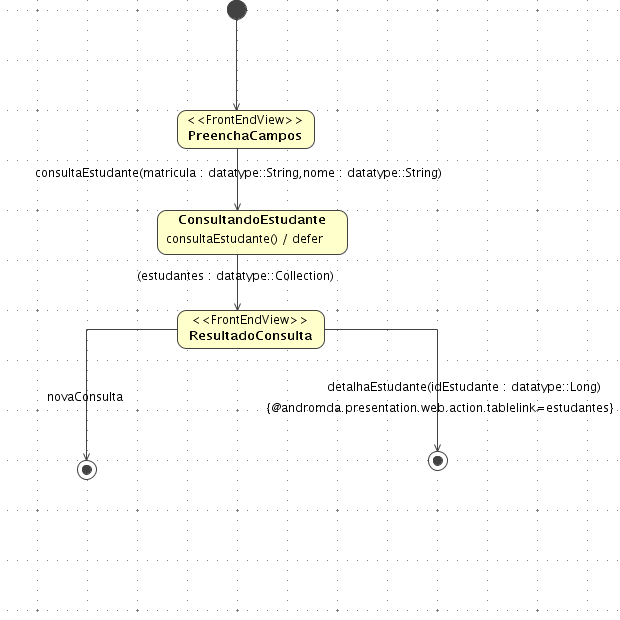
\includegraphics[width=350pt,height=300pt]{files/imgs/tutorial-mdarte-0028.png}
	\caption{Modelo do caso de uso Consulta Estudante.}
	\label{modelo_consulta_estudante}
\end{figure}

Abriremos a especificação da \texttt{transition} que sai da \texttt{front end
view} de nome \texttt{preencha os campos}, clicaremos no botão \texttt{edit}, no
\texttt{fieldset} \texttt{trigger}. Na aba \texttt{parameters}, da janela
\texttt{signal event specification}, que será aberta automaticamente, dê duplo
clique no nome do parâmetro \texttt{matricula} e será então aberta a
especificação do parâmetro. Selecione então a aba \texttt{tagged values},
selecione o \texttt{tagged value}
\texttt{@andromda.presentation.web.view.field.type} e clique no botão
\texttt{create value}. Selecione então a opção \texttt{autocomplete}, como na
imagem \ref{field_type_autocomplete}.

\begin{figure}[H]
	\centering
	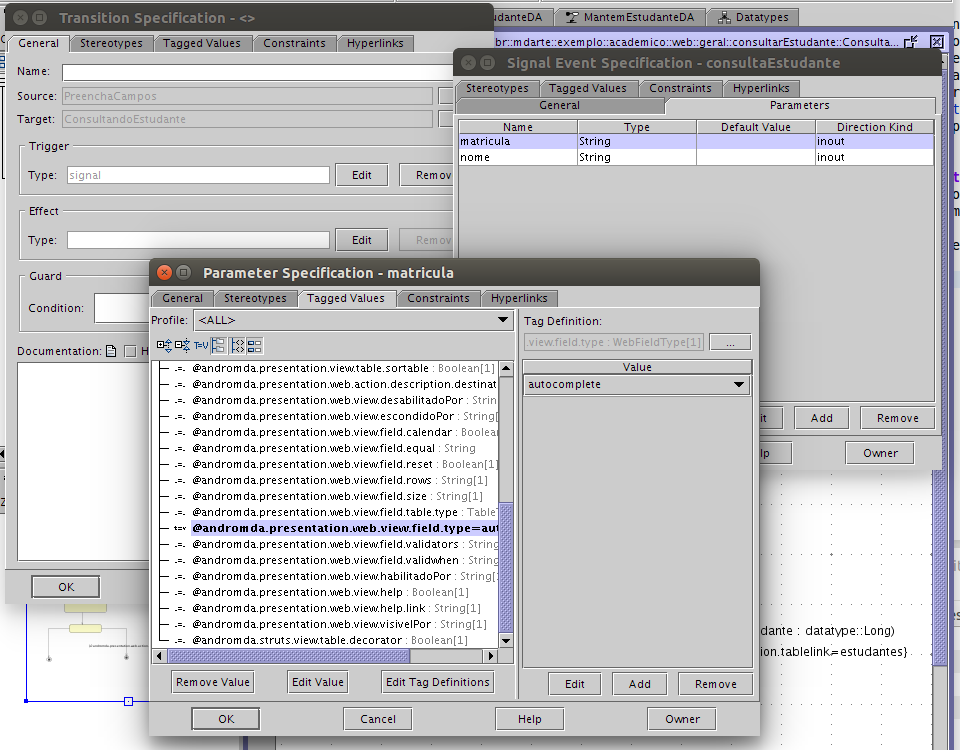
\includegraphics[width=350pt,height=300pt]{files/imgs/tutorial-mdarte-0027.png}
	\caption{Adicionando o field type 'autocomplete' à um campo da view.}
	\label{field_type_autocomplete}
\end{figure}

Agora executaremos o seguinte comando no terminal na raiz do projeto:
\begin{lstlisting}[language=bash]
maven mda -Dprojeto=sistemaacademico-geral-Estudante
\end{lstlisting}

Feito isto, o \texttt{MDArte} gerará automaticamente toda a estrutura
responsável por receber e tratar as requisições assíncronas para o preenchimento do
\texttt{autocomplete}, restando ao desenvolver apenas implementar no
\texttt{ControleImpl} a filtragem dos valores retornados, de acordo com o valor
do campo. Para isto, criaremos, na classe
\texttt{ConsultaEstudanteControleImpl}, um método seguindo o seguinte padrão 
\texttt{protected String[]
<nome-do-campo><nome-do-caso-de-uso>AutoComplete(java.lang.String query,
org.andromda.bpm4struts.ViewContainer container)}. Vejamos abaixo um exemplo de
implementação para o \texttt{autocomplete} do nosso campo de \texttt{matrícula}:

\lstinputlisting[language=java, frame=single, breaklines=true] {files/java/autocomplete.java}

Agora executaremos o seguinte comando para compilar e dar \texttt{deploy} no
\texttt{Sistema Acadêmico} :

\begin{lstlisting}[language=bash, frame=single, breaklines=true]
maven compile deploy
\end{lstlisting}

Feito isto, daremos \texttt{start} no \texttt{JBoss} e abriremos o sistema e
faremos login. Na tela \texttt{Preencha os Campos} do caso de uso
\texttt{Consulta Estudante} podemos agora verificar o \texttt{autocomplete}
funcionando, como na imagem \ref{exemplo_autocomplete}.

\begin{figure}[H]
	\centering
	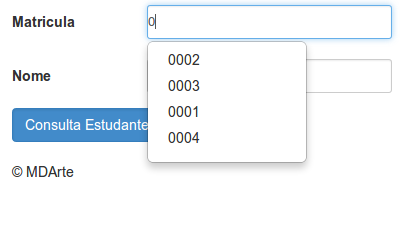
\includegraphics[width=350pt,height=300pt]{files/imgs/tutorial-mdarte-0029.png}
	\caption{Exemplo de autocomplete.}
	\label{exemplo_autocomplete}
\end{figure}
\section{Tabela assíncrona (JTable)}

Nesta seção veremos como implementar uma tabela \texttt{assíncrona}
(\texttt{JTable}) usando o \texttt{MDArte}. Para tal, vamos considerar como
ponto de partida o modelo do caso de uso \texttt{Consulta Estudante} conforme as
alterações feitas no tópico anterior. Certifique-se de ter removido o
estereótipo \texttt{«Manageable»} da classe \texttt{Estudante} no diagrama de
classes que descreve a \texttt{Camada de domínio}, a fim de evitar que o
\texttt{CRUD} seja re-gerado, sobrescrevendo assim as alterações que faremos.

Veremos agora, por subseções, algumas das funcionalidades disponíveis na tabela
assíncrona.

\subsection{Implementando filtragem assíncrona da tabela}
Nesta seção veremos como criar uma action ajax que reflita nos dados exibidos
por uma tabela ajax. A título de exemplo, faremos uma tela com um formulário e
um botão que, uma vez clicado, recarregará a tabela filtrando-a de acordo com os
dados do formulário. Tomaremos como base a tabela criada no exemplo de criação
de tabelas.

O modelo portanto começará assim:

\begin{figure}[H]
	\centering
	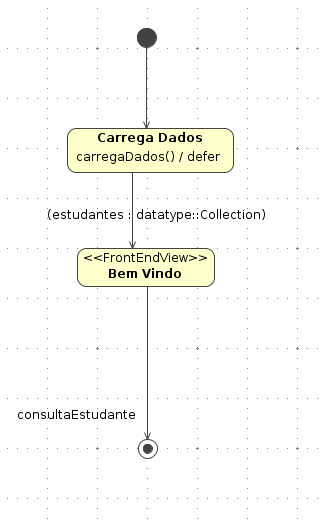
\includegraphics[width=180pt,height=260pt]{files/imgs/tutorial-mdarte-0040.png}
	\caption{Modelagem da filtragem assíncrona da tabela.}
	\label{modelando_filtragem_assincrona}
\end{figure}

Modelaremos então uma \texttt{transition} saindo da \texttt{FrontEndView} que
contém a nossa tabela e retornando para a mesma \texttt{view}, que será
interpretada pelo \texttt{MDArte} como uma ação assíncrona na \texttt{view}.
Abriremos então sua especificação e iremos na aba \texttt{tagged values} e
selecionaremos o \texttt{tagged value}
\texttt{@andromda.presentation.web.action.async.table} e daremos a ele o valor
\texttt{[nome-da-tabela]} (\texttt{estudantes}, nesse caso), esse \texttt{tagged
value} indica qual tabela será afetada pela ação assíncrona, nos permitindo ter
mais de uma de tabela assíncrona na mesma tela, tendo \texttt{actions} que
afetem somente uma tabela sem afetar a outra. Iremos então na aba
\texttt{general} e clicaremos no botão \texttt{edit} no \texttt{fieldset}
\texttt{'trigger'}, daremos o nome que desejarmos o \texttt{trigger} criado, no
exemplo fo idado o nome de \texttt{“filtrar”}, e selecionaremos seu tipo como
\texttt{signal}. Iremos então na aba \texttt{parameters}, ainda na especificação
do \texttt{trigger} e criaremos os parâmetros necessários para o processamento
da requisição, neste exemplo colocaremos só os parâmetros \texttt{matrícula} e
\texttt{nome}, a título de ilustração, e definiremos seus tipos como
\texttt{String}.

O modelo ficará assim:
\begin{figure}[H]
	\centering
	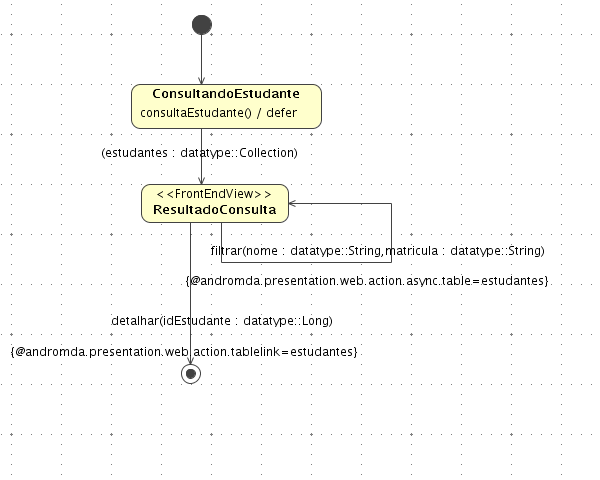
\includegraphics[width=340pt,height=300pt]{files/imgs/tutorial-mdarte-0036.png}
	\caption{Modelagem da filtragem assíncrona da tabela.}
	\label{modelando_filtragem_assincrona}
\end{figure}

Executaremos agora o seguinte comando para validar o modelo e regerar o
sistema:
\begin{lstlisting}[language=bash, frame=single, breaklines=true]
maven mda -Dprojeto=sistemaacademico-geral-Estudante
\end{lstlisting}

Agora adaptaremos, no \texttt{ControleImpl}, os métodos responsáveis pelo
carregamento da tabela, com a assinatura \texttt{public final Collection
load[nome-da-view][nome-da-tabela]Table}, e pelo retorno do número máximo de
elementos na mesma, com a assinatura \texttt{public final Integer
get[nome-da-view][nome-da-tabela]TableLength}, a fim de implementarmos o filtro.
Cada parâmetro da \texttt{trigger} pertencente à \texttt{transition} modelada
será adicionado, em ordem, à lista de parâmetros de cada método, logo antes do
parâmetro \texttt{ViewContainer container}. De acordo com o nosso exemplo, o
código ficará assim:
\lstinputlisting[language=java, frame=single, breaklines=true]{files/java/JTableFiltro.java}

Executaremos agora o seguinte comando para compilar e dar \texttt{deploy} no
sistema:
\begin{lstlisting}[language=bash, frame=single, breaklines=true]
maven compile deploy
\end{lstlisting}

Restartando o servidor e abrindo o caso de uso \texttt{Consulta Estudante},
veremos o resultado do que fizemos:
\begin{figure}[H]
	\centering
	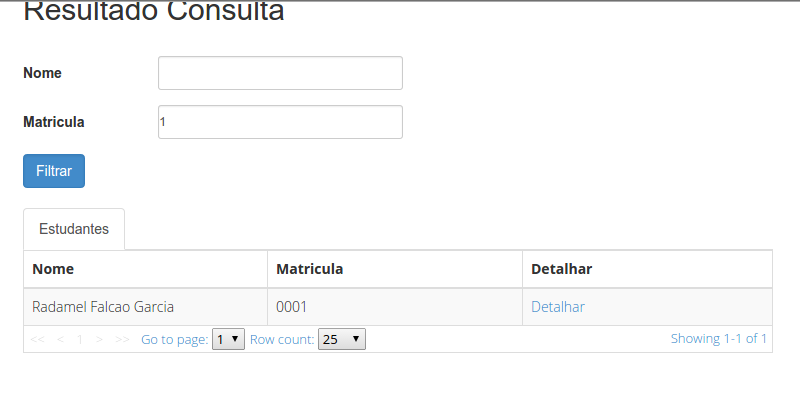
\includegraphics[width=340pt,height=300pt]{files/imgs/tutorial-mdarte-0042.png}
	\caption{Modelagem da filtragem assíncrona da tabela.}
	\label{modelando_filtragem_assincrona}
\end{figure}

\section{Criação de Componente customizado}

Nesta seção veremos como criar um campo customizado em uma tela. Iremos partir
do modelo de \texttt{CRUD} gerado automaticamente pelo \texttt{MDArte}, para a
entidade \texttt{Estudante}, e faremos as alterações necessárias para a criação
de um novo componente. O componente a ser desenvolvido, somente a título de
exemplo, será um campo texto com máscara para \texttt{CPF}.

Podemos ver o estado inicial do modelo na imagem \ref{modelo_consulta_estudante_custom}.

\begin{figure}[H]
	\centering
	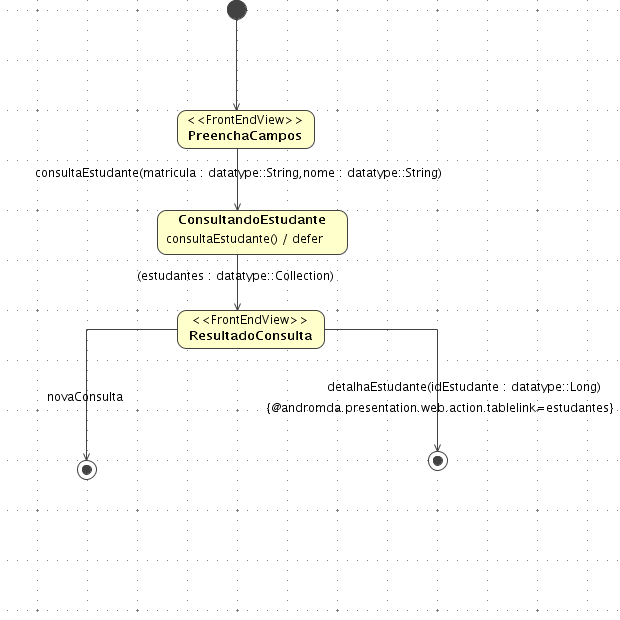
\includegraphics[width=350pt,height=300pt]{files/imgs/tutorial-mdarte-0028.png}
	\caption{Modelo do caso de uso Consulta Estudante.}
	\label{modelo_consulta_estudante_custom}
\end{figure}

Abriremos então a especificação da \texttt{transition}
\texttt{'consultaEstudante'}, clicaremos no botão \texttt{'edit'}, no
\texttt{fieldset} \texttt{'trigger'}, selecionaremos então a aba
\texttt{'parameters'}, da janela aberta quando clicamos o botão anterior, e
clicaremos então no botão \texttt{add}.

Preencheremos então os dados do campo conforme a imagem
\ref{dados_campo_custom_cpf}, SEM, no entanto, clicar no botão \texttt{Ok}.

\begin{figure}[H]
	\centering
	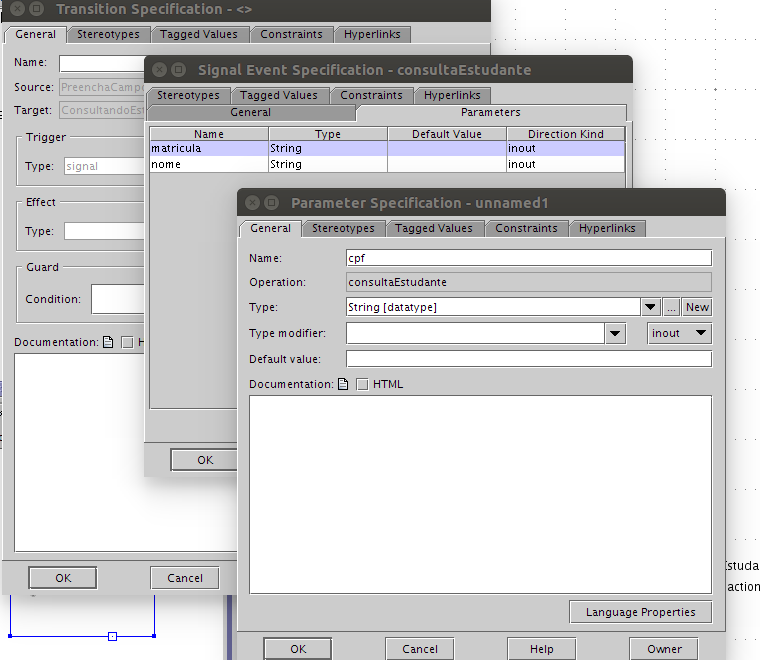
\includegraphics[width=350pt,height=300pt]{files/imgs/tutorial-mdarte-0033.png}
	\caption{Dados do campo 'cpf'.}
	\label{dados_campo_custom_cpf}
\end{figure}

Ainda na mesma janela, selecionaremos a aba \texttt{tagged values},
selecionaremos o \texttt{tagged value} 
\texttt{@andromda.presentation.web.view.field.type}, clicaremos no botão
\texttt{create value} e selecionaremos a opção \texttt{'custom'}, no campo
\texttt{combobox} que será exibido, como na imagem \ref{parametro_cpf_custom}.

\begin{figure}[H]
	\centering
	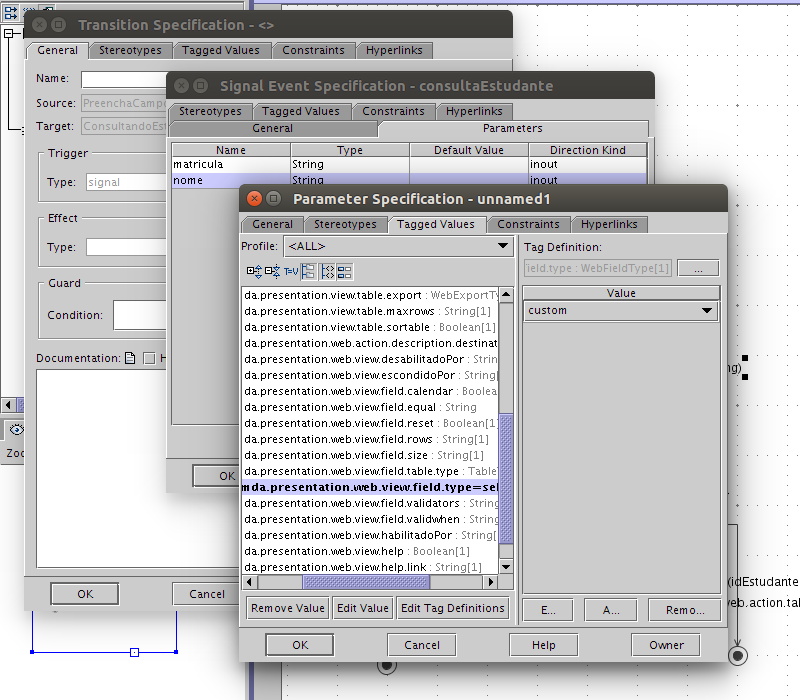
\includegraphics[width=350pt,height=300pt]{files/imgs/tutorial-mdarte-0034.png}
	\caption{Selecionando tipo custom para o campo 'cpf'.}
	\label{parametro_cpf_custom}
\end{figure}

Salvaremos então o modelo e digitaremos os seguintes comandos para regerar o
modelo:

\begin{lstlisting}[language=bash, frame=single, breaklines=true]
maven mda -Dprojeto=sistemaaacademico-geral-Estudante
\end{lstlisting}

Feito isto, o \texttt{MDArte} gerará um arquivo no padrão
\texttt{<nome-do-campo>.jsp}, neste caso, \texttt{cpf.jsp}, no caminho
\texttt{<nome-sistema>/web/<modulo-web>/src/jsp/<caminho-do-pacote-base>/web/<modulo-web>/<nome-caso-de-uso>},
mas você também pode encontrá-lo, no eclipse, através do comando
\texttt{ctrl+shift+r}, digitando o nome do arquivo na janela que é aberta por
esse comando.

Aberto o arquivo, adicionaremos a este o seguinte código \texttt{jsp}:

\lstinputlisting[language=html, frame=single, breaklines=true]{files/jsp/cpf.jsp}

O \texttt{html} adicionado será importado para a tela do sistema no espaço do
formulário dedicado ao campo \texttt{cpf}.

Adicionado o \texttt{jsp} do nosso componente, uma vez que se trata de um campo
de texto com um determinado comportamento (formatar a entrada no modelo do CPF),
precisamos agora adicionar um mecanismo de controle para o comportamento do
campo. Para tal, utilizaremos o \texttt{framework} para \texttt{javascript}
JQuery, uma vez que este já vem com o \texttt{MDArte}, além do fato de o
\texttt{JQuery} já possuir uma funcionalidade nativa que faça isso.

Para adicionar código \texttt{Javascript} manualmente a uma \texttt{view}
precisamos abrir o arquivo \texttt{<nome-da-view>-impl.js}, no mesmo caminho
do arquivo \texttt{jsp} alterado acima. O arquivo alterado é destinado ao código
adicionado pelo desenvolvedor para customizar o comportamento da aplicação, não
sendo sobrescrito durante a geração. Certifique-se, portanto, de estar
adicionando o seu código nestes pontos de implementação, a fim de não perdê-lo
na próxima geração.

Adicionaremos agora o seguinte código \texttt{JavaScript} ao arquivo
\texttt{preencha-campos-impl.js}:

\lstinputlisting[language=c, frame=single, breaklines=true]{files/js/preencha-campos-impl.js}
\section{Reformulação da View}
Nesta seção, trataremos da nova estrutura e organização da camada de visão do
MDArte.

A base da estrutura da \texttt{view} do MDArte encontra-se nos \texttt{layouts},
que são arquivos que definem a estrutura das páginas que definem, através da
definição de \texttt{tags} \texttt{html} e da importação demais arquivos
contendo partes menores da \texttt{view}.

O \texttt{layout} \texttt{default} do \texttt{MDArte} é definido nos arquivos de
nome \texttt{main-layout2.jsp}. Além disso, há também os arquivos
\texttt{main-layout-open.jsp}, responsável por definir o \texttt{layout} das
páginas que não estão submetidas à controle de acesso, e
\texttt{simple-layout.jsp}, que configura o \texttt{layout} de páginas simples
ou até mesmo de porções de hypertexto retornadas via \texttt{AJAX}.

Este conjunto de arquivos de \texttt{layout} é gerado \texttt{para cada módulo
Web} do sistema, a partir do \texttt{default} do sistema, dando liberdade ao
desenvolvedor de, se necessário, adaptar a aparência de cada módulo
independentemente.
